\subsection{Berechnung des Trägheitsmoments durch Approximation des Körpers}

\begin{figure}
\begin{minipage}{.49\textwidth}
    \centering
    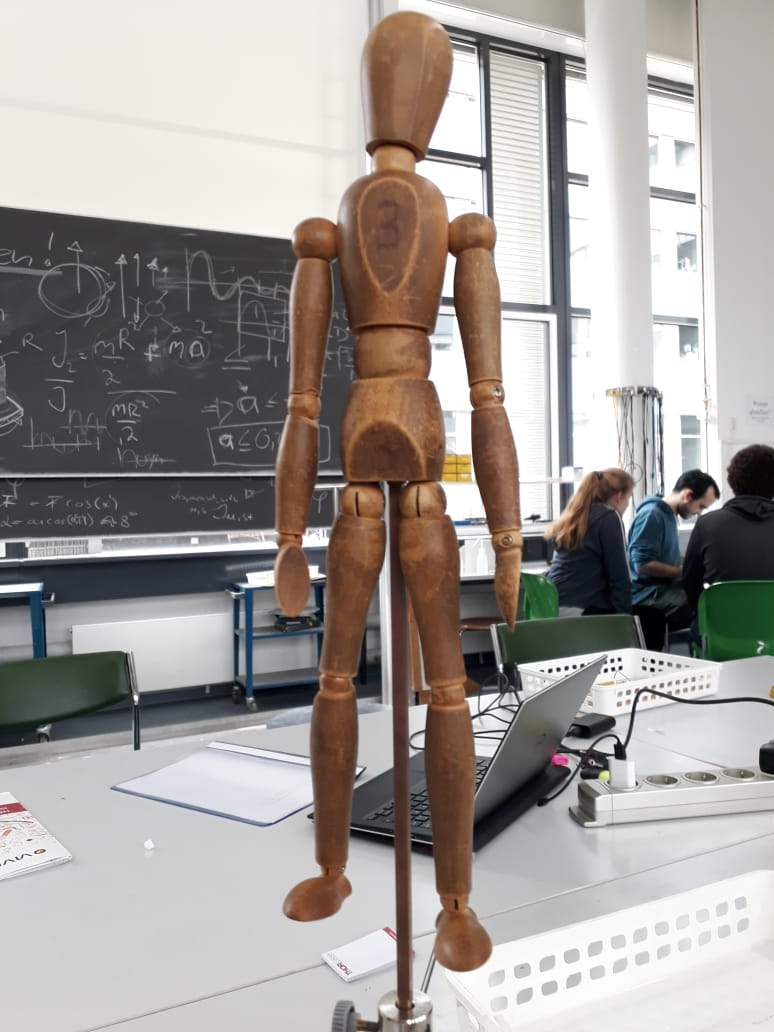
\includegraphics[scale=.28]{./Bilder/figur1.jpeg}
    \caption{Figur 1}
\end{minipage}
\begin{minipage}{.49\textwidth}
    \centering
    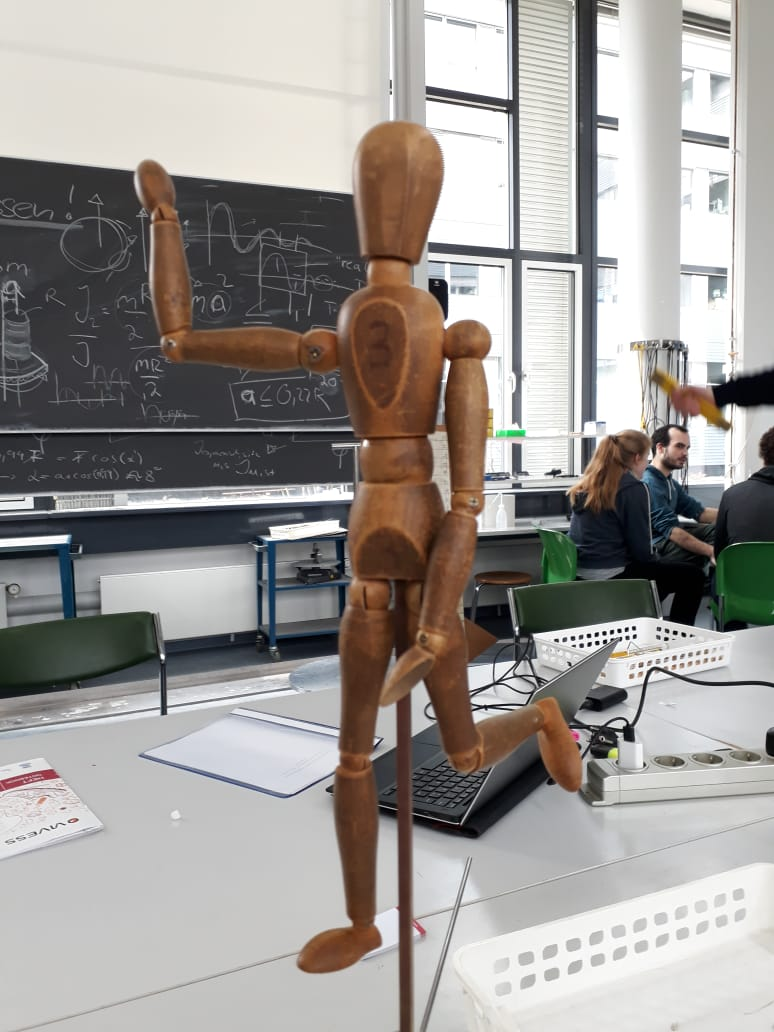
\includegraphics[scale=.28]{./Bilder/figur2.jpeg}
    \caption{Figur 2}
\end{minipage}
\end{figure}


Für Person 1 und Figur 1 errechnen wir ein theoretisches Trägheitsmoment von  $\unit[0.8]{kg\,m^2}$. Für Person 2 und Figur 2 erhalten wir einen Wert von $\unit[1.9]{kg\,m^2}$. 

